\subsection{fTools Plugin}\label{sec:ftools}

% when the revision of a section has been finalized, 
% comment out the following line:
\updatedisclaimer

The goal of the fTools python plugin is to provide a one-stop resource for
many common vector-based GIS tasks, without the need for additional software, 
libraries, or complex workarounds. It provides a growing suite of spatial 
data management and analysis functions that are both quick and functional. 

\minisec{Install the fTools Plugin}

To use the functionalities in QGIS, you must install the fTool python plugin
with the \mainmenuopt{Fetch Python Plugins} Installer (see 
Section \ref{sec:load_external_plugin}). Then select and load it 
with the Plugin Manager. Therefore click the menu \mainmenuopt{Plugins} > 
\mainmenuopt{Manage Plugins}, select \dropmenuopt{fTools} and click 
\button{OK}. A new menu \mainmenuopt{Tools} occurs in the menu bar with 
following features:

\minisec{Analysis tools}

\begin{table}[ht]\index{Analysis tools}
\centering
\caption{fTool analysis tools}\label{tab:ftool_analysis}\medskip
 \begin{tabular}{|p{0.3in}|p{1.2in}|p{4.7in}|}
 \hline \textbf{Icon} & \textbf{Tool} & \textbf{Purpose} \\
 \hline 
\includegraphics[width=0.7cm]{pointdistance} & Distance Matrix &
Measure distances between two point layers, and output results as a) Square
distance matrix, b) Linear distance matrix, or c) Summary of distances. Can
limit distances to the k nearest features. \\ 
 \hline 
\includegraphics[width=0.7cm]{sumlines} & Sum line length & Calculate
the total sum of line lengths for each polygon of a polygon vector layer. \\
 \hline 
\includegraphics[width=0.7cm]{pointpoly} & Points in polygon & Count
the number of points that occur in each polygon of an input polygon vector
layer. \\
 \hline 
\includegraphics[width=0.7cm]{listunique} & List unique values & List
all unique values in an input vector layer field. \\
 \hline 
\includegraphics[width=0.7cm]{fieldstats} & Basic statistic & Compute
basic statistics (mean, std dev, N, sum, CV) on an input field. \\ 
 \hline 
\includegraphics[width=0.7cm]{nearestneigh} & Nearest Neighbor analysis
& Compute nearest neighbour statistics to assess the level of clustering in a
point vector layer. \\
 \hline 
\includegraphics[width=0.7cm]{meancoords} & Mean coordinate(s) &
Compute either the normal or weighted mean center of an entire vector layer,
or multiple features based on a unique ID field. \\ 
 \hline 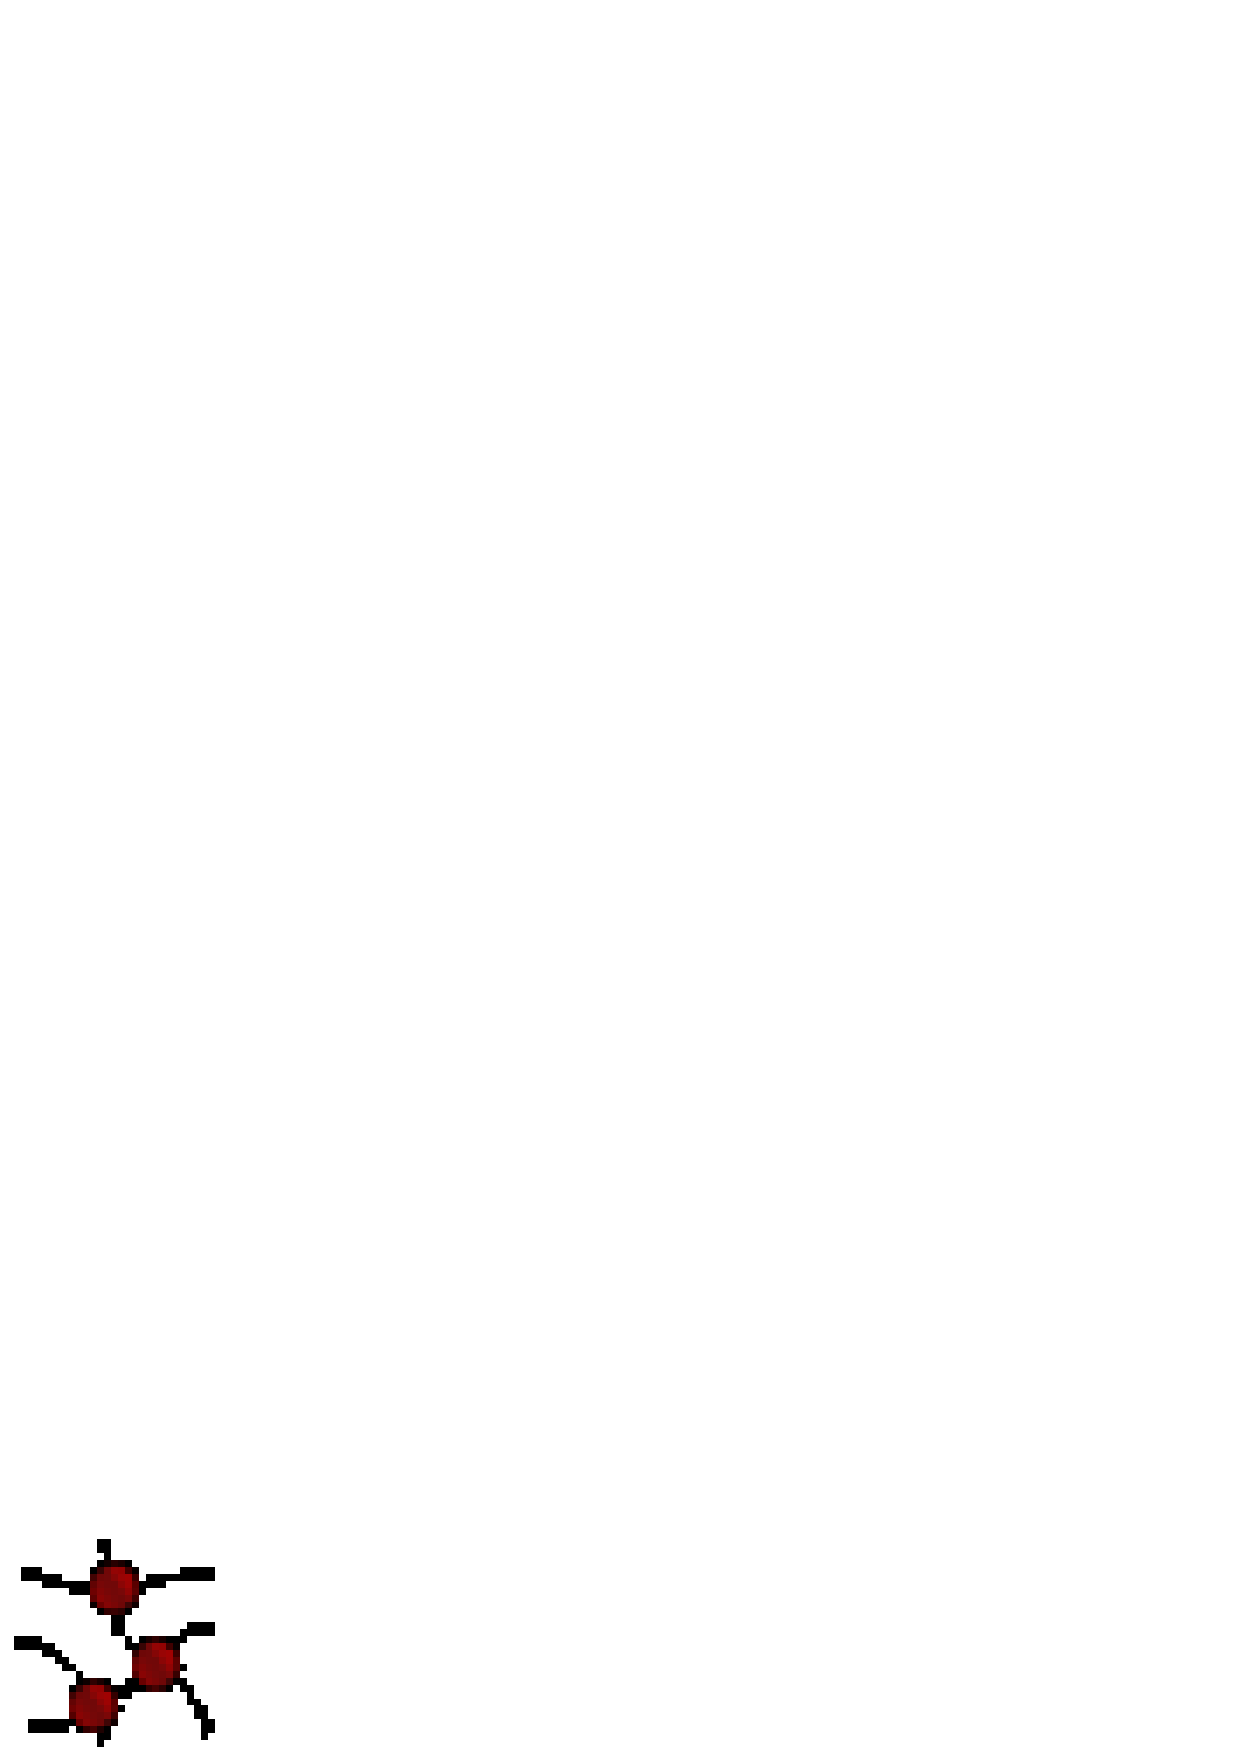
\includegraphics[width=0.7cm]{intersectlines} & Line intersections &
Locate intersections between lines, and output results as a point shapefile.
Useful for locating road or stream intersections, ignores line intersections
with length > 0. \\
 \hline
\end{tabular}
\end{table}

\minisec{Sampling tools}

\begin{table}[ht]\index{Sampling tools}
\centering
\caption{fTool sampling tools}\label{tab:ftool_sampling}\medskip
 \begin{tabular}{|p{0.3in}|p{1.3in}|p{4.6in}|}
 \hline \textbf{Icon} & \textbf{Tool} & \textbf{Purpose} \\
 \hline 
\includegraphics[width=0.7cm]{random} & Random selection & Randomly 
select n number of features, or n percentage of features \\
 \hline 
\includegraphics[width=0.7cm]{selectsubset} & Random selection within 
subsets & Randomly select features within subsets based on a unique ID field. \\
 \hline 
\includegraphics[width=0.7cm]{randompoints} & Random points & Generate 
pseudo-random points over a given input layer. \\
 \hline 
\includegraphics[width=0.7cm]{regularpoints} & Regular points & Generate 
a regular grid of points over a specified region and export them as a point shapefile. \\
 \hline 
\includegraphics[width=0.7cm]{vectorgrid} & Vector grid & Generate a 
line or polygon grid based on user specified grid spacing. \\
 \hline 
\includegraphics[width=0.7cm]{selectlocation} & Select by location & 
Select features based on their location relative to another layer to form a 
new selection, or add or subtract from the current selection. \\
 \hline
\end{tabular}
\end{table}

\minisec{Geoprocessing tools}

\begin{table}[ht]\index{Geoprocessing tools}
\centering
\caption{fTool geoprocessing tools}\label{tab:ftool_geoprocessing}\medskip
 \begin{tabular}{|p{0.3in}|p{0.8in}|p{5.1in}|}
 \hline \textbf{Icon} & \textbf{Tool} & \textbf{Purpose} \\
 \hline 
\includegraphics[width=0.7cm]{multiconvex} & Convex hull & Create 
minimum convex hull(s) for an input layer, or based on an ID field. \\
 \hline 
\includegraphics[width=0.7cm]{dynamicbuffer} & Buffer & Create 
buffer(s) around features based on distance, or distance field. \\
 \hline 
\includegraphics[width=0.7cm]{intersect} & Intersect & Overlay 
layers such that output contains areas where both layers intersect. \\
 \hline 
\includegraphics[width=0.7cm]{union} & Union & Overlay layers such 
that output contains intersecting and non-intersecting areas. \\
 \hline 
\includegraphics[width=0.7cm]{symdiff} & Symetrical difference & 
Overlay layers such that output contains those areas of the input and 
difference layers that do not intersect. \\
 \hline 
\includegraphics[width=0.7cm]{clip} & Clip & Overlay layers such 
that output contains areas that intersect the clip layer. \\
 \hline 
\includegraphics[width=0.7cm]{erase} & Difference & Overlay layers 
such that output contains areas not intersecting the clip layer. \\
 \hline 
\includegraphics[width=0.7cm]{dissolve} & Dissolve & Merge features 
based on input field. All features with indentical input values are combined 
to form one single feature. \\
 \hline
\end{tabular}
\end{table}

\newpage

\minisec{Geometry tools}

\begin{table}[ht]\index{Geometry tools}
\centering
\caption{fTool geometry tools}\label{tab:ftool_geometry}\medskip
 \begin{tabular}{|p{0.3in}|p{1.2in}|p{4.8in}|}
 \hline \textbf{Icon} & \textbf{Tool} & \textbf{Purpose} \\
 \hline 
\includegraphics[width=0.7cm]{checkgeometry} & Check geometry & 
Check polygons for intersections, closed-holes, and fix node ordering. \\
 \hline 
\includegraphics[width=0.7cm]{calcgeom} & Export/Add geometry 
columns & Add vector layer geometry info to point (XCOORD, YCOORD), 
line (LENGTH), or polygon (AREA, PERIMETER) layer. \\
 \hline 
\includegraphics[width=0.7cm]{centroids} & Polygon centroids & 
Calculate the true centroids for each polygon in an input polygon layer. \\
 \hline 
\includegraphics[width=0.7cm]{simplify} & Simplify geometry & 
Generalise lines or polygons with a modified Douglas-Peucker algorithm. \\
 \hline 
\includegraphics[width=0.7cm]{multitosingle} & Multipart to 
singleparts & Convert multipart features to multiple singlepart features. 
Creates simple polygons and lines. \\
 \hline 
\includegraphics[width=0.7cm]{singletomulti} & Singleparts to 
multipart & Merge multiple features to a single multipart feature based 
on a unique ID field. \\
 \hline 
\includegraphics[width=0.7cm]{polystolines} & Polygons to lines 
& Convert polygons to lines, multipart polygons to multiple singlepart lines. \\
 \hline 
\includegraphics[width=0.7cm]{extractnodes} & Extract nodes & 
Extract nodes from line and polygon layers and output them as points. \\
 \hline
\end{tabular}
\end{table}

\minisec{Data management tools}

\begin{table}[ht]\index{Data management tools}
\centering
\caption{fTool data management tools}\label{tab:fTool_data_management}\medskip
 \begin{tabular}{|p{0.3in}|p{1.3in}|p{4.6in}|}
 \hline \textbf{Icon} & \textbf{Tool} & \textbf{Purpose} \\
 \hline 
\includegraphics[width=0.7cm]{project} & Export to projection & 
Project features to new CRS and export as new shapefile. \\
 \hline 
\includegraphics[width=0.7cm]{define} & Define projection & 
Specify the CRS for shapefiles whose CRS has not been defined. \\
 \hline 
\includegraphics[width=0.7cm]{joinattr} & Join attributes & Join 
additional attributes to vector layer attribute table and output results 
to a new shapefile. Additional attributes can be from a vector layer or 
stand-alone dbf table. \\
 \hline 
\includegraphics[width=0.7cm]{spatialjoin} & Join attributes by 
location & Join additional attributes to vector layer based on spatial 
relationship. Attributes from one vector layer are appended to the attribute 
table of another layer and exported as a shapefile \\
 \hline 
\includegraphics[width=0.7cm]{vectorsplit} & Split vector layer & 
Split input layer into multiple separate layers based on input field. \\
 \hline
\end{tabular}
\end{table}



